% Source: Code/CommonSenseCarolina/legislation-thumbnails.tex
\documentclass[border=0pt]{standalone}
\usepackage{tikz}
\usepackage{fontspec}
\usetikzlibrary{calc,positioning}

\definecolor{garnet}{HTML}{73000A}
\definecolor{black90}{HTML}{363636}
\definecolor{black70}{HTML}{5C5C5C}
\definecolor{black50}{HTML}{A2A2A2}
\definecolor{warmgrey}{HTML}{676156}
\definecolor{sandstorm}{HTML}{FFF2E3}

\setmainfont{Georgia}
\setsansfont{Helvetica}

\begin{document}

% ============================================================
% BILL — White background
% ============================================================
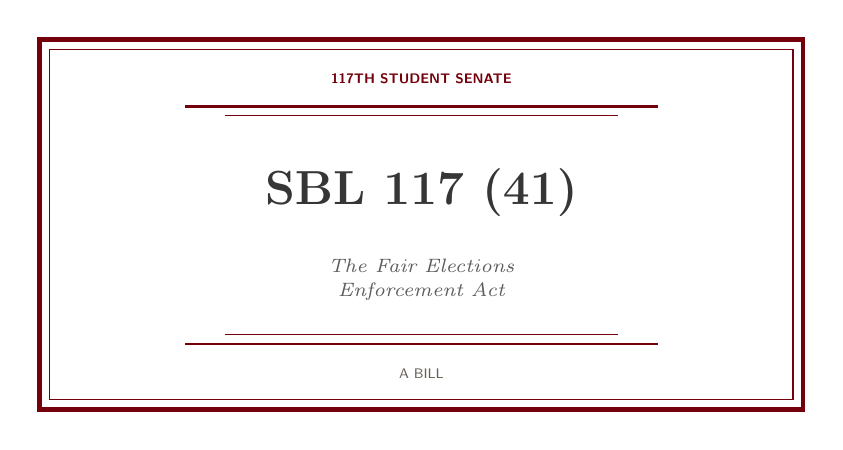
\begin{tikzpicture}
  \fill[white] (0,0) rectangle (10,5);
  \draw[garnet, line width=1.5pt] (0.15,0.15) rectangle (9.85,4.85);
  \draw[garnet, line width=0.4pt] (0.28,0.28) rectangle (9.72,4.72);

  \draw[garnet, line width=0.8pt] (2,4.0) -- (8,4.0);
  \draw[garnet, line width=0.3pt] (2.5,3.88) -- (7.5,3.88);

  \node[garnet, font=\sffamily\fontsize{5.5}{7}\selectfont\bfseries]
    at (5,4.35) {117TH STUDENT SENATE};

  \node[black90, font=\fontsize{18}{20}\selectfont\bfseries]
    at (5,2.9) {SBL 117 (41)};

  \node[black70, font=\itshape\fontsize{7}{9}\selectfont, text width=6cm, align=center]
    at (5,1.8) {The Fair Elections\\Enforcement Act};

  \draw[garnet, line width=0.3pt] (2.5,1.1) -- (7.5,1.1);
  \draw[garnet, line width=0.8pt] (2,0.98) -- (8,0.98);

  \node[warmgrey, font=\sffamily\fontsize{4.5}{6}\selectfont]
    at (5,0.6) {A BILL};
\end{tikzpicture}
\hspace{0.5cm}
% ============================================================
% RESOLUTION — Sandstorm background
% ============================================================

\begin{tikzpicture}
  \fill[sandstorm] (0,0) rectangle (10,5);
  \draw[garnet, line width=1.5pt] (0.15,0.15) rectangle (9.85,4.85);
  \draw[garnet, line width=0.4pt] (0.28,0.28) rectangle (9.72,4.72);

  \draw[garnet, line width=0.8pt] (2,4.0) -- (8,4.0);
  \draw[garnet, line width=0.3pt] (2.5,3.88) -- (7.5,3.88);

  \node[garnet, font=\sffamily\fontsize{5.5}{7}\selectfont\bfseries]
    at (5,4.35) {117TH STUDENT SENATE};

  \node[black90, font=\fontsize{18}{20}\selectfont\bfseries]
    at (5,2.9) {SBL 117 (XX)};

  \node[black70, font=\itshape\fontsize{7}{9}\selectfont, text width=7cm, align=center]
    at (5,1.8) {Defend Student Organizations Against\\Discriminatory Funding Models};

  \draw[garnet, line width=0.3pt] (2.5,1.1) -- (7.5,1.1);
  \draw[garnet, line width=0.8pt] (2,0.98) -- (8,0.98);

  \node[warmgrey, font=\sffamily\fontsize{4.5}{6}\selectfont]
    at (5,0.6) {A RESOLUTION};
\end{tikzpicture}
\hspace{0.5cm}
% ============================================================
% RECOMMENDATION — Garnet background
% ============================================================

\begin{tikzpicture}
  \fill[garnet] (0,0) rectangle (10,5);
  \draw[sandstorm, line width=1.5pt] (0.15,0.15) rectangle (9.85,4.85);
  \draw[sandstorm, line width=0.4pt] (0.28,0.28) rectangle (9.72,4.72);

  \draw[sandstorm, line width=0.8pt] (2,4.0) -- (8,4.0);
  \draw[sandstorm, line width=0.3pt] (2.5,3.88) -- (7.5,3.88);

  \node[sandstorm, font=\sffamily\fontsize{5.5}{7}\selectfont\bfseries]
    at (5,4.35) {117TH STUDENT SENATE};

  \node[white, font=\fontsize{18}{20}\selectfont\bfseries]
    at (5,2.9) {SBL 117 (01)};

  \node[sandstorm, font=\itshape\fontsize{7}{9}\selectfont, text width=7cm, align=center]
    at (5,1.8) {Transparency of Strom Thurmond Wellness\\Center Occupancy Data};

  \draw[sandstorm, line width=0.3pt] (2.5,1.1) -- (7.5,1.1);
  \draw[sandstorm, line width=0.8pt] (2,0.98) -- (8,0.98);

  \node[sandstorm, font=\sffamily\fontsize{4.5}{6}\selectfont, opacity=0.7]
    at (5,0.6) {A RECOMMENDATION};
\end{tikzpicture}

\end{document}
